%%%%%%%%%%%%%%%%%%%%%%%%%%%%%%%%%%%%%%%%%%%%%%%%%%%%
% This will help you in writing your homebook
% Remember that the character % is a comment in latex
%
% chapter 1
\chapter{Introduction}
\label{chap1}
%%%%%%%%%%%%%%%%%%%%%%%%%%%%%%%%%%%%%%%%%%%%%%%%%%%%%%%%%%%
% you can organize a chapter using sections -> \section{Simulating an inverter}
% or subsections -> \subsection{simulating a particular type of inverter}
%%%%%%   First section
The goal of this laboratory is to design and synthesize a RISC-V-lite processor. 
The ISA of this processor includes:
\begin{itemize}
    \item R-Type instructions;
    \item I-Type instructions;
    \item S-Type instructions;
    \item SB-Type instructions;
    \item UJ-Type instructions;
    \item U-Type instructions.
\end{itemize}

The format of the instructions is summarized in the following image.
\begin{figure}[!h]
\centering
    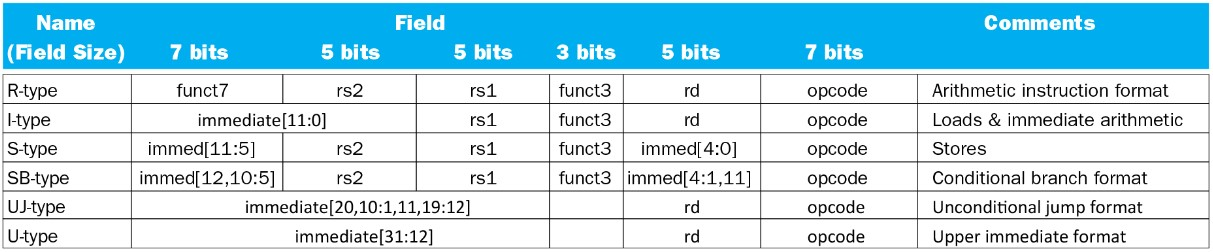
\includegraphics[width=\linewidth]{chapters/chap1images/Immagine 2022-02-14 214305.jpg}
    \caption{\textbf{Instruction Format}}
\end{figure}

In particular, the processor is required to support a subset of the RV32I ISA, which corresponds to:
\begin{itemize}
    \item \textbf{Arithmetic:}
    \begin{itemize}
        \item \textbf{add:} R-Type instruction performing the addition between the source registers.
        \item \textbf{addi:} I-Type instruction performing the addition between a source register and an immediate value.
        \item \textbf{auipc:} U-Type instruction that adds the content of the program counter with an immediate value.
        \item \textbf{lui:} U-Type instruction that stores the immediate value in the destination register.
    \end{itemize}
    \item \textbf{Branches:}
    \begin{itemize}
        \item \textbf{beq:} SB-Type instruction used to update the value of the program counter if the content of the two source registers is equal.
    \end{itemize}
    \item \textbf{Loads:}
    \begin{itemize}
        \item \textbf{lw:} I-Type instruction used to read a word from memory, computing the address using the immediate value. The word is stored in the destination register.
    \end{itemize}
    \item \textbf{Shifts:}
    \begin{itemize}
        \item \textbf{srai:} I-Type instruction performing the arithmetic right shift of the content of the source register, by a number of positions corresponding to the immediate value.
    \end{itemize}
    \item \textbf{Logical:}
    \begin{itemize}
        \item \textbf{andi:} I-Type instruction performing the logical AND between the source register and the immediate value.
        \item \textbf{xor:} R-Type instruction performing the logical XOR between the two source registers.
    \end{itemize}
    \item \textbf{Compare:}
    \begin{itemize}
        \item \textbf{slt:} R-Type instruction that compares the content of the two source registers.
    \end{itemize}
    \item \textbf{Jump and link:}
    \begin{itemize}
        \item \textbf{jal:} J-Type instruction performs a jump to the instruction indicated by the sum between the PC and the immediate value. The value of the PC before the jump, 
        increased by 4, is stored in the destination register.
    \end{itemize}
    \item \textbf{Stores:}
    \begin{itemize}
        \item \textbf{sw:} S-Type instruction that stores the value of the source register in the memory, whose address is computed using the immediate value.
    \end{itemize}
\end{itemize}

    The processor uses a 32-bit parallelism and is composed of 5 pipeline stages, instruction fetch, instruction decode, execute, access memory and write back.
    The stages will be described in the following chapters, as well as the techniques utilized to avoid hazards and in general guarantee the correct operation of the processor. 
    Finally, the memories are not included in the design, instead they are implemented in the testbench for simulation purposes.

    The following image shows the schematic of the RISCV processor.
    \begin{figure}[!h]
        \centering
            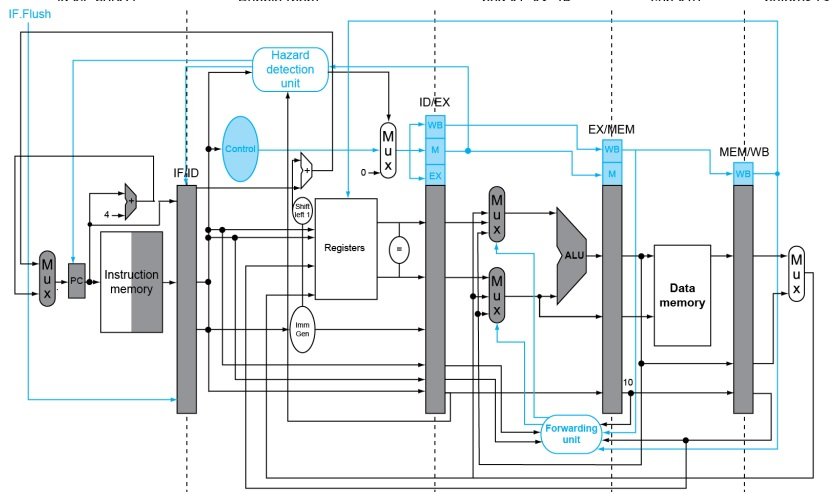
\includegraphics[width=\linewidth]{schematic/schematic.jpg}
            \caption{\textbf{Schematic of the design}}
    \end{figure}
        